\documentclass[a4paper,12pt]{article}
\usepackage[T1]{fontenc}
\usepackage[utf8]{inputenc}
\usepackage{lmodern}
\usepackage[spanish]{babel}
\usepackage{textcomp}
\usepackage{amsmath}
\usepackage{amsfonts}
\usepackage[framed,numbered,autolinebreaks]{mcode}
\usepackage{amssymb}
\usepackage{graphicx}
\usepackage{caption}
\usepackage{subcaption}
\usepackage{float}
\usepackage{color}
\usepackage{mcode}
\usepackage[left=2cm,right=2cm,top=2cm,bottom=2cm]{geometry}
\usepackage{fancyhdr}
\usepackage[hidelinks]{hyperref}
\title{Puntos extra examen parcial}
\author{
  Cabrera López Oscar Emilio
}

\pagestyle{fancy}
\fancyhf{}
\lhead[]{}
\chead[]{}
\rfoot{\thepage}
\lfoot[]{}
\cfoot[]{}

\linespread{1.3}

\renewcommand\headrule
{{\color[RGB]{98,36,35}%
    \hrule height 2pt
    width\headwidth
    \vspace{1.3pt}%
    \hrule height 1pt
    width\headwidth
  }}
  \addto\captionsspanish{\def\tablename{Tabla}}%imprime Tabla en lugar de Cuadro
  %%
  \spanishdecimal{.}


\begin{document}
\thispagestyle{fancy}
\maketitle
\newpage
\tableofcontents
\newpage

\section{Ejercicio 1}
Determine la clasificación del siguiente sistema en tiempo en tiempo continuo:
\[ y(t) = u(x(t)) \]
Clasificación: 1,3,6,7,8.
\begin{enumerate}
    \item No lineal: sin importar la entrada que tenga, no cumplirá ni linealidad ni homogeneidad.
    \item Estático por lo tanto causal.
    \item Variante en el tiempo.
    \item Estable BIBO: no importa la entrada. la respuesta será siempre estará entre 0 y 1.
\end{enumerate}
\section{Ejercicio 2}
A partir de la respuesta al impulso determine la función de transferencia y el diagrama de bloques del sistema.
\[ h(t)=\left(\frac{3}{2}e^{-4t}-\frac{1}{2}e^{-2t}\right)u(t) \]
\[ \mathcal{L}\left\{h(t)=\left(\frac{3}{2}e^{-4t}-\frac{1}{2}e^{-2t}\right)u(t)\right\} \]
\[ H(s) = \frac{\frac{3}{2}}{s+4} - \frac{\frac{1}{2}}{s+2} \]
\[ H(s) = \frac{s+5}{(s+2)(s+4)} = \frac{s+5}{s^2+6s+8} \]
\[ s^2Y(s)+6sY(s)+8Y(s) = sX(s)+5X(s)  \]
\[ \frac{8Y(s)}{s^2}+\frac{6Y(s)}{s}+Y(s) = \frac{5X(s)}{s^2}+\frac{X(s)}{s} \]
\[ Y(s) = -\frac{8Y(s)}{s^2}-\frac{6Y(s)}{s}+\frac{5X(s)}{s^2}+\frac{X(s)}{s} \]
\begin{figure}[H]
  \begin{center}
    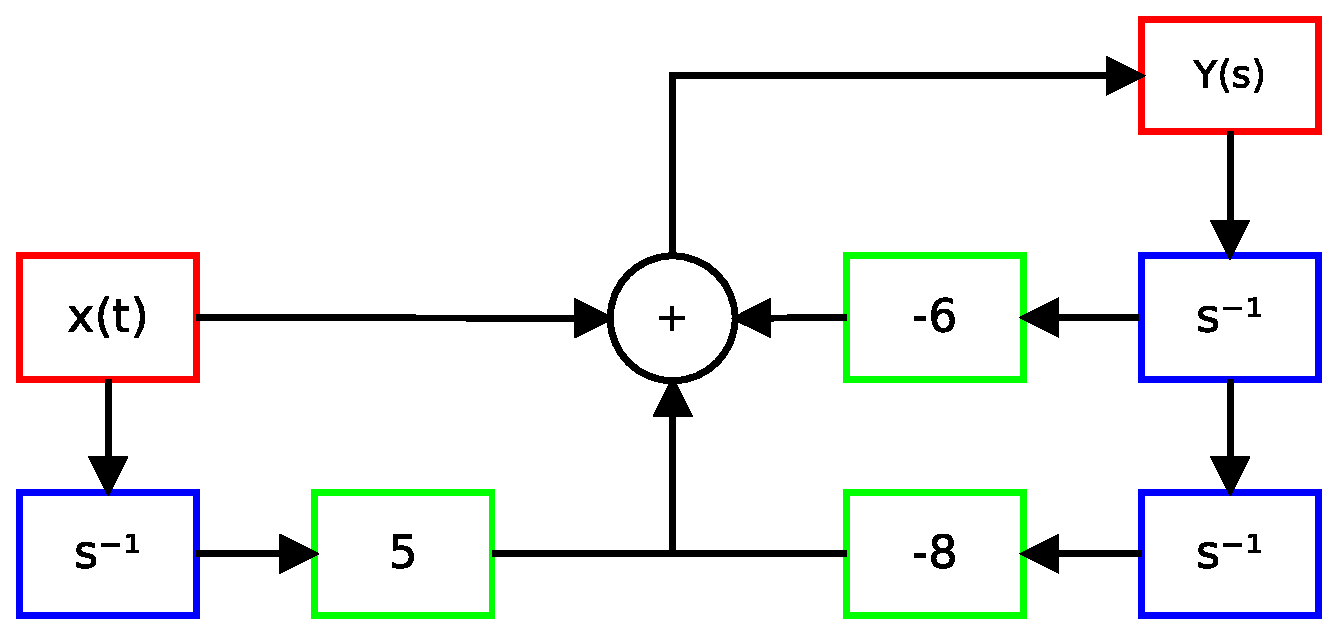
\includegraphics[width=0.8\textwidth]{Diagrama}
    \caption{Diagrama de bloques del sistema}
    \label{fig:dia}
  \end{center}
\end{figure}
\section{Ejercicio 3}
Investigue la propiedad de la convolución con funciones singulares y con ella obtenga la convolución de
\[ u(t)\ast u_{1}(t) \]
La propiedad de convolución con el doblete unitario nos dice que
\[ \int_{\infty}^{\infty}x(\tau)\delta'(t-\tau)dt = -x'(t) \]
esto se puede generalizar como 
\[ \int_{\infty}^{\infty}x(\tau)\delta^{(n)}(t-\tau)dt = (-1)^nx^{(n)}(t) \]
Por lo tanto
\[ u(t)\ast u_{1}(t) = -\delta(t) \]
\end{document}
